Dessa forma, STALLINGS (2017) apresenta uma proposta de arquitetura básica de GPU baseada na microarquitetura Fermi da NVIDIA (lançada em abril de 2010 e com processo de fabricação de 40nm e 28nm), pois apresenta uma documentação completa e detalhada e segue como ponto de partida para a compreensão da arquitetura de GPUs.

\subsection{Arquitetura geral da NVIDIA Fermi}

A figura \ref{arq:fermi:1} mostra uma visão geral da GPU da arquitetura da Fermi da NVIDIA. Pode ser encontrado na figura, 8 blocos de multiprocessadores de \textit{streaming} (MS) acima e oito abaixo. No centro encontra-se uma memória \textit{cache} L2 que recebe dados das 16 MS. Os retângulos na parte de cima e de baixo de cada MS são onde os registradores e a memória compartilhada L1 estão localizadas. Nas laterais contabilizam seis interfaces DRAM E/S e possuem interface de memória de 64 bits, cada, totalizando 384 bits para a interface da DRAM GDDR5. Outro bloco é a interface de \textit{host}, que é responsável pela conectividade PCIe entre a GPU e CPU. O bloco restante é o escalonador global GigaThread e é responsável pela distribuição dos blocos de \textit{thread} para os escalonadores \textit{warp }do MS.


\begin{figure}
\centering
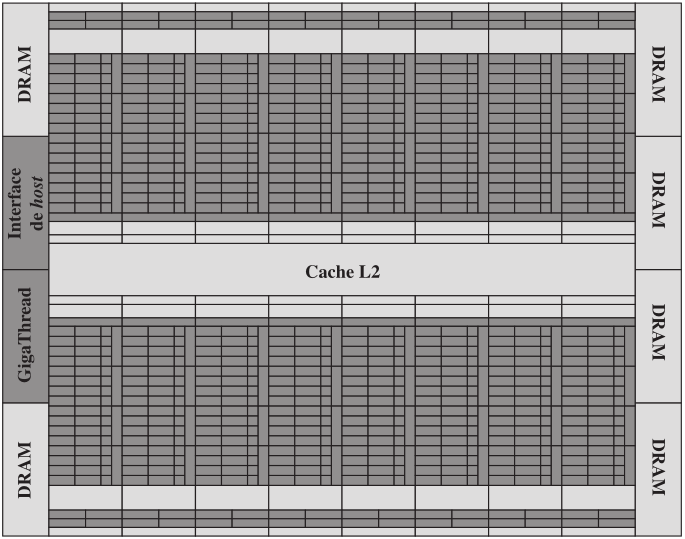
\includegraphics[width=8.4cm]{arquitetura.png} 
\caption{Arquitetura da MS da NVIDIA Fermi. (STALLINGS, 2017)} 
\label{arq:fermi:1}
\end{figure}

\subsection{Detalhes da arquitetura do multiprocessador de \textit{streaming}}

De acordo com a figura \ref{arq:fermi:2} detalhando um único MS da microarquitetura Fermi da NVIDIA, pode-se contabilizar  os seguintes componentes: 32 cores de processadores de GPU (cores CUDA); 2 escalonadores \textit{warp} e unidade de despacho´; 16 unidades de carga/armazenamento; 4 unidades de funções espaciais (SFU); banco de registradores de 32k x 32 bits; memória cache L1 compartilhada de 64 kB no total. Em seguida, cada um desses componentes serão detalhados.

\subsubsection{Escalonador \textit{warp} duplo}

A unidade GigaThread distribui os blocos de thread para os MSs. O escalonador de \textit{warp} duplo vai separar cada bloco de thread que está processando em warps (grupo de 32 threads, com IDs de threads consecutivas que começam no mesmo endereço inicial). A partir da emissão de um warp, cada thread terá seu contador de endereço de instrução e conjunto de registradores, permitindo desvios e execução independente de threads no MS.

\subsubsection{\textit{Cores} CUDA}

Cada core tem dois pipelines ou datapath separados: uma unidade pipeline de inteiro (INT) e uma unidade de pipeline de ponto flutuante (PF). Porém apenas um desses datapath podem ser usados durante um único ciclo de clock. A unidade INT comporta 32 bits, 64 bits e precisão estendida para operações de inteiros e lógicas bit a bit. A unidade PF apresenta uma operação de precisão única, sendo necessárias dois cores para uma operação de PF de precisão dupla, levando o dobro do tempo.

\subsubsection{SFU}

Cada MS contém quatro SFUs. Estas apresentam operações como seno, cosseno, recíproca e raiz quadrada que são executadas em um ciclo de clock. Caso 32 threads solicitem as SFUs, leva-se 8 ciclos de clock para completar um warp.

\subsubsection{Unidades de carga/armazenamento}

Calculam a fonte e o endereço de destino para um único thread por ciclo de clock. Os endereços são para a cache ou a DRAM a partir dos quais os threads querem ler ou escrever dados.

\subsubsection{Registradores, memória compartilhada e cache L1}



\begin{figure}
\centering
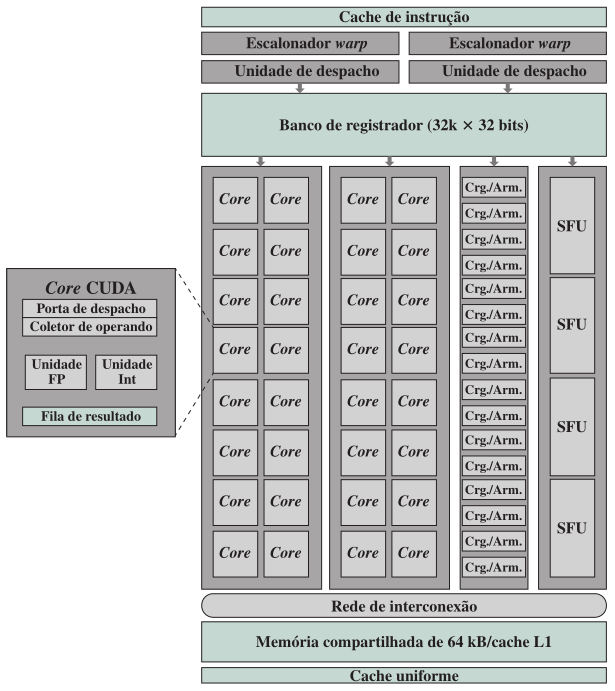
\includegraphics[width=8.4cm]{arquitetura_MS.png} 
\caption{Arquitetura de um único processador de streaming. (STALLINGS, 2017)} 
\label{arq:fermi:2}
\end{figure}